\documentclass[a4paper,12pt]{article}

% Pakete laden
\usepackage[T1]{fontenc}
\usepackage[utf8]{inputenc}
\usepackage[ngerman]{babel}
%\usepackage{lmodern}
\usepackage{geometry}
%\usepackage{setspace}
\usepackage{graphicx}
%\usepackage{amsmath}
%\usepackage{amssymb}
%\usepackage{booktabs}
%\usepackage{natbib}
%\usepackage{tikz}
%\usepackage{caption}
%\usepackage{listings}
%\usepackage{ragged2e}
%\usetikzlibrary{positioning}
%\usetikzlibrary{shapes}
%\usepackage{afterpage}
%\usepackage{float}
%\usepackage{titlesec}
\usepackage{hyperref}%hyperref links

\usepackage{fancyhdr}%footer
\usepackage{graphicx}%images
\usepackage{wrapfig}%images in text
\usepackage{adjustbox}
\usepackage{pdfpages}  % Include this line to use the pdfpages package
\usepackage{longtable}%for table that spread over multiple pages
\usepackage{float}%fix figure position
%\usepackage{lastpage}
\usepackage[yyyymmdd]{datetime}%display the date better
\renewcommand{\dateseparator}{-}

%\bibliographystyle{unsrt}





% Kopfzeile
\pagestyle{fancy}
\fancyhf{}
\fancyhead[L]{\includegraphics[width=5 cm]{OST_Logo.png}}
\fancyhead[R]{Maschinentechnik | Innovation}
\geometry{headsep=1.6cm}%sonst fängt das logo zu weit unten

% Fusszeile 
\rfoot{Seite \thepage}
%\rfoot{\thepage}
\renewcommand{\footrulewidth}{0pt}
\fancyfoot[L]{Peter Kuhn} % author on the left
\fancyfoot[C]{Bachelorarbeit FS 2024} % title in the c enter




% Titelblatt
\begin{document}


\begin{titlepage}
  \end{titlepage}
% Import the PDF
%toChange

\includepdf{Titelseite.pdf}
%import something from scribus


\pagestyle{empty}
\section*{Abstract}


\iffalse

Dazu habe ich unterschiedliche  physikalische Wirkprinzipien getestet. 
Die vielversprechendste Technik basiert auf einem Water Indikator Tape- das ursprünglich für die Elektronik entwickelt wurde und  das visuell ausgewertet wird.

 Für eine definierte Zeitspanne wird das Tape auf die Schneeoberfläche gelegt. Anschliessend wird es fotografiert. Die Auswertung erfolgt durch visuelle und digitale Analyse.
Das Produkt durchlief 5 Iterationen. Die entwickelte Messtechnik zeigt die Fähigkeit, die Interaktion des gefrorenen und des flüssigen Wassers mit dem Tape zu erfasseberfasst werden.

Weitere Optimierung und Testung ist erforderlich, um die Genauigkeit und Präzision des Sensors zu gewährleisten.

Dies ist Voraussetzung dafür, den Sensor in der Zukunft zu einem marktfähigen Produkt weiter entwicklen zu können.

Die Ergebnisse dieser Arbeit können einen Beitrag zur Weiterentwicklung von Messmethoden für den LWC im Schnee leisten. Eine  verbesserte Vorhersage von Gleitschneelawinen ermöglicht adäquate Reaktionen auf dieses Naturereignis. 




in dieser produktentwicklungsaufgabe wurde eine Innovativer sensor entwickelt um den Liquid water Contet von schnee zu messen.

dazu wurden verschiedene physikalische wirkprinzipien getesten. die vielversprechendste technik in der ein Water indikator Tape aus der qualitassicherung im elektronikbrachnche visuell auswertet wird, wurde uber 5 iterationen entwickelnt um die interaktion des schnees und Taps zu verstehen.


Die messmethode zeigt die fahigkeiten den lwc von schnee zu erfassen. bis jetzt ist es aber noch nicht sicher ob die prazision und genauigkeit ausreichend ist um in ein produkt umgesetzt zu werden.


In dieser Arbeit wurde ein innovativer Sensor zur Messung des Flüssigwassergehalts (Liquid Water Content, LWC) in Schnee entwickelt. Verschiedene physikalische Prinzipien wurden getestet, um die beste Methode zur Bestimmung des LWC zu identifizieren. Die vielversprechendste Technik erwies sich als der Einsatz eines Wasserindikatorbands aus der Qualitätssicherung in der Elektronikbranche, welches visuell ausgewertet wird. Über fünf Iterationen hinweg wurde der Sensor weiterentwickelt, um die Interaktion zwischen Schnee und dem Indikatorband besser zu verstehen.

Die Auswertung erfolgt durch visuelle und digitale Analyse des 3M 5559 Water Indikator Tapes. Das Tape, das bei Kontakt mit Wasser rot wird, wird für definierte Zeitspannen auf die Schneeoberfläche gelegt und anschließend fotografiert. Die visuelle Beurteilung erfolgt durch die einfache Betrachtung der roten Verfärbung auf dem Tape. Für eine präzisere Analyse wird die Bildverarbeitung eingesetzt, bei der Software den Anteil der roten zu weißen Fläche berechnet, um den Flüssigwassergehalt zu quantifizieren.

Die entwickelte Messtechnik zeigt die Fähigkeit, den LWC im Schnee zu erfassen, jedoch ist die Präzision und Genauigkeit der Messungen noch nicht ausreichend, um den Sensor als marktfähiges Produkt zu etablieren. Weitere Optimierungen und umfangreiche Tests sind erforderlich, um die Zuverlässigkeit und Praktikabilität des Sensors zu gewährleisten. Die Ergebnisse dieser Arbeit liefern einen wichtigen Beitrag zur Weiterentwicklung von Messmethoden für den LWC im Schnee und könnten zukünftig zur Verbesserung der Vorhersage und Prävention von Gleitschneelawinen beitragen.

\fi

\subsection*{Beschreibung der Abkürzungen}
\begin{acronym}[XXXXX]
    \setlength{\itemsep}{-\parsep}
    \acro{BA}{Bachelorarbeit}
    \acro{LWC}{Liquid Water Content}
    \acro{SLF}{Schweizerisches Institut für Schnee- und Lawinenforschung}
    \acro{IPEK}{Institut für Produktentwicklung}
    \acro{TRL}{Technology Readiness Level}
    \acro{ML}{Maschinelles Lernen}
    \acro{IR}{Infra Rot}
    \acro{FDM}{Fused Deposition Modeling}
    \acro{FS}{Fruhlings Semester}
    \acro{OST}{Ost schweizer fachhochschule}
    \acro{MHz}{mega Herz}
    \acro{GPS}{gobal positioning system}
    \acro{Mri}{magnetic resonacn imaging}
    \acro{Tape}{Water indicator tape 5559 von 3M}
    \acro{CAD}{computer aided design}
    \acro{RGB}{Rot Grun blau}
    \acro{DB}{Daten Bank}
    \acro{xps}{extruded polystyrene}
\end{acronym}

% Inhaltsverzeichnis
\tableofcontents
%\pagenumbering{Roman}
\newpage
\pagestyle{fancy}

\setcounter{page}{1}
\section{Einleitung}
Ziel dieser Arbeit ist, einen Sensor zu entwickeln, der flüssiges Wasser im Schnee misst.

Das flüssige Wasser im Schnee ist ein entscheidender Parameter um das Verhalten des Schnees an einem lawinen gefährdeten Hang  vorherzusagen. Seit 40 Jahren wird das Thema erforscht,  und es gibt unterschiedliche Methoden das heterogene Gemisch aus festen, flüssigen und gasförmigen Stoffen, diesen Schaum aus Eis, Wasser und Luft zu messen.

Die vorhandenen Geräte nutzen unterschiedliche Ansätze, haben aber teils  Nachteile zum Beispiel dass sie das Verhältnis von flüssigem Wasser zum Schnee nicht in einem Arbeitsschritt erfassen.

Ich habe verschiedene theoretische Ansätze der Produktentwicklung im Verlauf der Bachelorarbeit genutzt.

Um den Sensor herzustellen habe ich entsprechend der agilen hardware Entwicklung möglichst rasch Iterationen von Sensoren als Produkt hergestellt, getestet und angepasst.

\iffalse
ziel dieser Arbeit ist die entwicklung eines innovativen sensors um die scheefeuchtigkeit zu messen.

Die schneefeuchtigkeit ist ein entscheidenen Parameter um Gleitschneelawinen abzuschetzten. seit 40 jahren ist wird Thema beforscht. Es gibt verschiedenste Techniken um den Schaum aus Eis, Wasser und Luft zu messen. heutige Produkte konnen den LWC messen, haben aber verschiedene schwerwigeende nachteile.

um dieses Produktentwicklung an zu gehen werden verschiedene techniken der Produktentwicklung eingesetzt. um ein sensor zu erreichen der einsatztfahig ist, wurde nach aglier hardware entwicklung moglichst schnell Itterationen von sensoren entwickelt.

\fi


\subsection{Lawinen in der Schweiz}

\subsection{Endziel des Arbeit}

\subsection{User Story}

\subsection{Anforderungen}

\subsection{Planung der Arbeit}

\section{Liquid Water Content}
\subsection{Physicalische Prinzipien}

\subsection{Kommerzielle Produkte}

\subsection{Publizierte Methoden}

\subsection{Methoden in der Vorstudie}

\section{Vorstudie}

\subsection{3M 5559 Water Indikator Tape}

\subsection{Voltcarft}

\subsection{Laser Refraktion, Reflezion}

\section{Funktionsmuster}

\subsection{Funktionsweise}

\subsection{Testkriterien}

\subsection{Montage des Funktionsmusters}

\subsection{Ergebnisse der Versuche}

\subsection{Vergleich der Ergebnisse mit Denometer}

\subsection{Verbesserungsmöglichkeiten des Funktionsmusters}

\newpage
\section{Ausblick}
\subsection{Presönliche Erfahrunng}

\subsection{Fazit}

\subsection{Ausblick}
Der weitere Verlauf der Forschung sollte darauf abzielen, die Präzision und Genauigkeit der Schneemessung zu erhöhen sowie die Anwendbarkeit des Systems in verschiedenen Umgebungen zu testen. Dabei sollten auch mögliche Verbesserungen im Hinblick auf die Automatisierung der Messungen und die Reduzierung des Arbeitsaufwands berücksichtigt werden.

Eine entscheidende Fragestellung besteht darin, die beobachtete Varianz in den Messungen zu verstehen. Es ist wichtig zu klären, ob diese Varianz auf Unterschiede im Liquid Water Content (LWC) des Schnees zurückzuführen ist oder ob sie einen Effekt der Messung selbst darstellt. Um eine statistisch fundierte Aussage treffen zu können, sollten über 30 Messungen von vergleichbaren Schneeproben durchgeführt werden.

Um die statistische Basis der Datenbank zu verbessern, sollten über 1000 Messungen mit dem Tape und etablierten LWC-Messwerten durchgeführt werden. Dadurch können die Daten analysiert, validiert und das Messsystem weiterentwickelt werden.


\newpage
% Literaturverzeichnis
%\bibliography{mybibliography}
\section{Literaturverzeichnis}



\begin{thebibliography}{9}

\bibitem{hypecycle} \url{https://www.gartner.com/en/articles/what-s-new-in-the-2023-gartner-hype-cycle-for-emerging-technologies}{Gartner Hype Cycle for Emerging Technologies 2023}, abgerufen am 19.12.2023

\bibitem{TempLink}  \url{https://www.schweizer-fn.de/stoff/waermedehnung/waermedehnung.php}{Temperature Expansion Tutorial}, abgerufen am 19.12.2023

\bibitem{SchwindungLit}   Christian Bonten. \textit{Kunststofftechnik: Einführung und Grundlagen}. Carl Hanser Verlag GmbH \& Co. KG, München, 3. aktualisierte edition, 2020.

\bibitem{VorlesungSML} Badertscher, H.: Vorlesung Statistical Machine Learning 2023
\bibitem{VorlesungKT} Ehrig, F. und Andere: Vorlesung Konstruieren mit Kunststoffen 2023
\bibitem{VorlesungDB} Schwab, J.: Vorlesung Datenbanksysteme 1 2023
\bibitem{VorlesungWah} Tietje, O.:Vorlesung Wahrscheinlichkeit und Messdaten 2022
\bibitem{VorlesungPyt} Malacarne S.:Vorlesung Python 2023
\bibitem{MAJaps} Hollender, J.: Vorhersage der Qualitätsmerkmale von Spritzgussbauteilen nach 24h anhand von Korrelationsmodellen 2021, unveröffentlichte Masterarbeit an der OST, Betreuer: Frank Ehrig
\bibitem{MAGew} Stocker, C.: Datengetriebene Prädiktion des Bauteilgewichts von Spritzgiessbauteilen 20221, unveröffentlichte Semesterarbeit an der OST, Betreuer: Frank Ehrig
\bibitem{SwissAI} \url{https://www.swissinfo.ch/eng/business/swiss-initiative-aims-for-global-leadership-in-ai/49029736}, abgerufen am 19.12.2023
\bibitem{VorlesungMess} Šeatović, D.: Vorlesung Messtechnik 2022
\bibitem{ChatGPT} ChatGPT
\bibitem{GPT4All} GPT4All mit Mistral OpenOrca LLM
\bibitem{WH} \url{https://www.wh.group/en/services/ruby/}
\bibitem{NewsP} \url{https://www.plasticstoday.com/injection-molding/how-artificial-intelligence-is-transforming-injection-molding}
\bibitem{NatureP} \url{https://www.nature.com/articles/s41598-023-48679-0}
\bibitem{ieeeP} \url{https://ieeexplore.ieee.org/document/8369500}
\bibitem{katulu} \url{https://katulu.io/en/solutions/briefs/ai-based-injection-molding/}

\end{thebibliography}



\newpage
\section{Erklärung zur Urheberschaft}


Ich erkläre hiermit, dass ich die vorliegende Arbeit ohne Hilfe Dritter angefertigt habe. Ich habe nur die Hilfsmittel benutzt, die ich angegeben habe. Gedanken, die ich aus fremden Quellen direkt oder indirekt übernommen habe, sind kenntlich gemacht. Die Arbeit wurde bisher keiner anderen Prüfungsbehörde vorgelegt und auch noch nicht veröffentlicht.

KI-Einsatz ohne Kennzeichnungspflicht

Ich bin mir bewusst, dass die Nutzung maschinell generierter Texte keine Garantie für die Qualität von Inhalten und Text gewährleistet. Ich versichere daher, dass ich den Text generierender KI-Tools lediglich als Hilfsmittel bedient habe und in der vorliegenden Arbeit meinen gestalterischen Einfluss überwiegt. Ich verantworte die Übernahme jeglicher von mir verwendeter maschinell generierter Textpassagen vollumfänglich selbst. Ich versichere, dass ich keine KI-Schreibwerkzeuge verwendet habe, deren Nutzung der Prüfer / die Prüferin explizit schriftlich ausgeschlossen hat.



Ort/Datum: Rapperswil, 2024 \\
Unterschrift:\\
Peter Kuhn


\newpage
\listoffigures


\listoftables % Tabellenverzeichnis erstellen
\newpage
\section{Digitaler Anhang}

\subsection*{Lebenslauf}
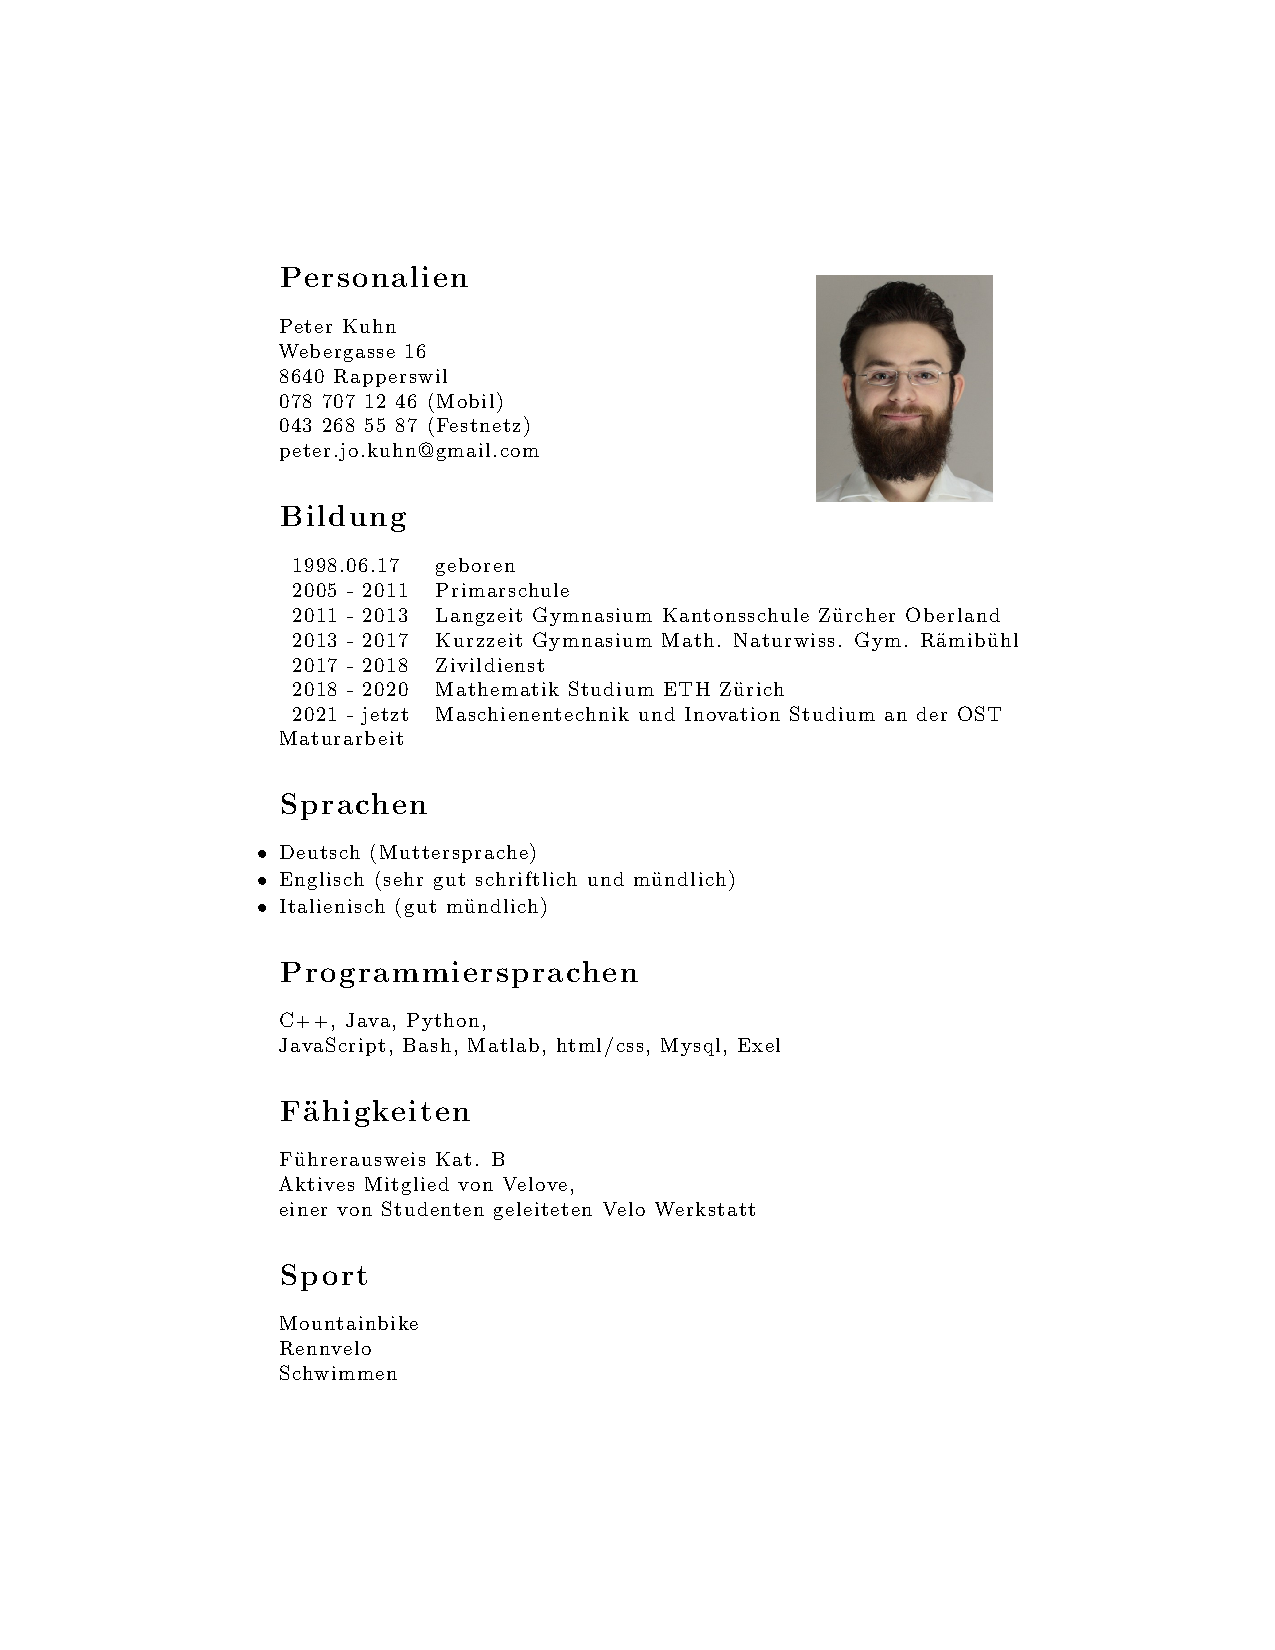
\includepdf{lebenslauf-2.pdf}


\end{document}
